\documentclass[11pt,a4paper]{article}
\usepackage{graphicx}
\usepackage[utf8]{inputenc}     %% european characters can be used (Linux)
\usepackage[T1]{fontenc}   %% get hyphenation and accented letters right
\usepackage{mathptmx}      %% use fitting times fonts also in formulas
\usepackage{linguex}       %% for linguistics glosses
\usepackage[round,colon]{natbib} %% for authornames with years for in-text references
\bibliographystyle{author1}
% do not change these lines:
\pagestyle{empty}                %% no page numbers!
\usepackage[left=35mm, right=35mm, top=15mm, bottom=20mm, noheadfoot]{geometry}
%% please don't change geometry settings!


\begin{document}
\thispagestyle{empty}

\title{\textbf{A Public POS-tagged Portuguese Language Corpus Built From
               Wikipedia Articles}}
\author{anonymous author\\
anonymous institution\\
anonymous@anonymous.org}
%\author{Álvaro Justen \quad Flávio Amieiro \quad Renato Rocha Souza \quad
%        Flávio Codeço Coelho\\
%Fundação Getúlio Vargas\\
%\{alvaro.justen,flavio.amieiro,renato.souza,fccoelho\}@fgv.br}

\date{}
\maketitle\thispagestyle{empty}

\section{Introduction}
There are some Portuguese part-of-speech tagged corpora freely available in the
Web, like MacMorpho, Floresta, Tycho Brahe and others. There are also some
closed/payed, like Parole. There is a scarcity of large, freely available,
part-of-speech tagged corpora in Portuguese and high-accuracy part-of-speech
taggers licensed as free software (one of the most accurate, PALAVRAS, is
closed-source software). With this in mind we looked for a large document
corpus that could be tagged and made available to serve as a base for new
research in Portuguese language processing.

Our goal was to use the best tools available to us to tag the entire Portuguese
Wikipedia and, knowing that the computational power and know-how needed to tag
such a large corpus is beyond the reach of many researchers, release our work
in a way it could be used by anyone, with hopes of encouraging further research
in the area.

\section{Choosing the Corpus}

Wikipedia is a collaborative multilingual (currently, 285
languages) encyclopedia, that has more than 25 million articles, written by
more than 100,000 active volunteers around the globe, the 5th most visited site
in the world. Its content is available through a Creative Commons license
(CC-BY-SA), so anyone already has permission to use, modify and
distribute it, without needing to ask for. For those reasons it has been used
for a myriad of research in varied fields such as Artificial Intelligence,
Statistics and Natural Language Processing.

Portuguese Wikipedia has more than 750,000 articles. It provides us with a
large corpus, with multiple authors and that spans many different knowledge
areas and writing styles.
%TODO: falar da licença do corpus que estamos disponibilizando: CC-BY-SA
% It also allows derivative works to be made available
% under a free license.


\section{Methodology}

\subsection{Extracting data}

Wikipedia regularly exports full dumps of their Portuguese version. We've
downloaded the version containing only current page revisions, then extracted
all desired pages (removing discussion, user and other meta-pages).
After having all titles and wikitext, we converted it to plain text. Tables,
images, lists and references were removed -- just plain text remained.

In total, 755,680 articles were processed, ranging from zero -- for pages
entirely composed of tables, lists or images -- to almost 47,000 tokens. Figure
\ref{fig:token_histogram} shows a token count histogram of the entire corpus.

%Text lengths
%  max=263557.0
%  avg=1221.03242607
%  stddev=3312.86714229
%Token counts
%  max=46923.0
%  avg=223.675451722
%  stddev=599.480419626

\begin{figure}[h]
\centerline{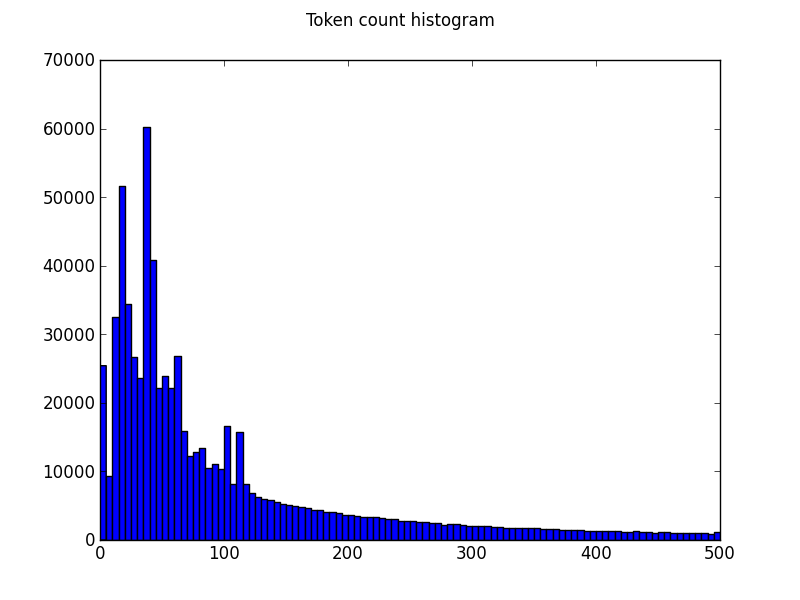
\includegraphics[width=10cm]{token_count_histogram.png}}
{\bf \caption{Token count histogram}
\label{fig:token_histogram}}
\end{figure}


\subsection{Tagging}

The final extracted data was submitted PyPLN\citep{pypln} using its HTTP API.
PyPLN is a free software platform for distributed Natural Language Processing
capable of handling large amounts of data. PyPLN performs a series of analyses
on the submitted documents, including part-of-speech tagging.


For this analyses we modified our PyPLN instances to use
PALAVRAS\citep{palavras}, a closed-source part-of-speech tagger based on a
Constraint Grammar Framework, to which we obtained a license.


All pages were tagged in a cluster of 3 machines, each of them with 16 cores
and 128GiB of memory. PyPLN distributed the jobs (tokenizing, tagging etc.)
among the cluster automatically.  The time to tag each document ranged from a
few milliseconds (for really small documents) up to 82 seconds, in an average
of 1.135 seconds.



\subsection{Exporting}

After processing every Portuguese Wikipedia page, we filtered out obvious
noises such as pages with no text remaining after the removal of tables, lists
and images (in a total of 19,398).

NLTK is one of the most used tools for NLP. We decided to make this corpus
available in a format NLTK can read. The Portuguese Wikipedia corpus (plain
text and tagged text) is distributed in such a way any NLTK user can use it
without any extra work.

%\section{Future works}
%\begin{itemize}
%    \item train taggers with tagged data (and compare them)
%    \item export wikipedia in a RESTful HTTP API (with PyPLN)
%    \item automate the process of tagging the entire corpus to update it easily
%    \item tag wikipedia in other languages
%    \item per-portal corpus
%\end{itemize}

\section{Conclusion}

We provide the tagged corpus for download in the format used by the popular
Natural Language Toolkit\citep{NLTK} and also make it available on
PyPLN's demonstration website, so researchers can navigate through the
documents and visualize the tagged data in a easy-to-use Web interface and also
download individual document data and analyses.

%\section{Keywords}
%natural language processing, Wikipedia, corpus linguistics, part-of-speech
%tagging, NLTK, Palavras, Python, free software, creative commons


\begin{thebibliography}{00}
\addcontentsline{toc}{chapter}{References}

\bibitem[\protect\citename{Coelho \bgroup et al.\egroup}, 2013]{pypln}
Flávio Codeço Coelho, Renato Rocha Souza, and Álvaro Justen. Pypln: a natural
language processing pipeline in python. page 6838. Euroscipy, 2012c. URL
http://www.euroscipy.org/talk/6838

\bibitem[\protect\citename{Bick}, 2000]{palavras}
Eckhard Bick. The Parsing System "Palavras": Automatic Grammatical Analysis of Portuguese in a Constraint Grammar Framework. Aarhus University Press, 2000.

\bibitem[\protect\citename{Bird}, 2009]{NLTK}
Bird, Steven, Edward Loper and Ewan Klein. Natural Language Processing with
Python. O’Reilly Media Inc, 2009

%\bibitem[\protect\citename{CC-BY-SA}]{\url{https://en.wikipedia.org/wiki/Wikipedia:Text_of_Creative_Commons_Attribution-ShareAlike_3.0_Unported_License}}

\end{thebibliography}

\end{document}
